\documentclass[12pt]{article}
\usepackage[letterpaper,margin=1in]{geometry}
\usepackage{amsmath,amsfonts,amssymb}
\usepackage{setspace}
\usepackage{fancyhdr}
\usepackage{lastpage}
\usepackage{chngpage}
\usepackage[protrusion=true,expansion,kerning]{microtype}
\usepackage[lofdepth,lotdepth]{subfig}
\usepackage{url}
\usepackage{algpseudocode}
\usepackage{comment}
\usepackage{pgf}
\usepackage{tikz}
\usetikzlibrary{arrows,automata}
\usepackage[color=yellow!20]{todonotes}

\usepackage[absolute,overlay]{textpos}
  \setlength{\TPHorizModule}{1mm}
  \setlength{\TPVertModule}{1mm}

% adjust margins:
\topmargin=-0.25in
\evensidemargin=0in
\oddsidemargin=0in
\textwidth=6.5in
\textheight=8.5in
\headsep=0.25in

% document-specific information
\newcommand{\docTitle}{Attention Plots}
\newcommand{\docSubTitle}{}
\newcommand{\docDate}{April 10, 2013}
\newcommand{\docClass}{}
\newcommand{\docInstructor}{}
\newcommand{\authorName}{}

% header and footer
\pagestyle{fancy}
\lhead{\docTitle}
\chead{}
\rhead{\docDate}   
\lfoot{}
\cfoot{}
\rfoot{\emph{Page\ \thepage\ of\ \pageref{LastPage}}}                          
\renewcommand\headrulewidth{0.4pt}
\renewcommand\footrulewidth{0.4pt}

\renewcommand{\labelenumiii}{\arabic{enumiii}.}
\renewcommand{\labelenumiv}{\arabic{enumiv}.}

\begin{document}
\begin{center}
Mean squared error averaged over all testing data versus (constant) precision (in bits) of the network. Error is on a log scale. For a given set size $s$, network is trained on $2^{s-3}$ of the $2^s$ possible inputs (selected at random), tested on the remaining inputs. Learning rate $\eta=4.0$, 400 iterations over training data.
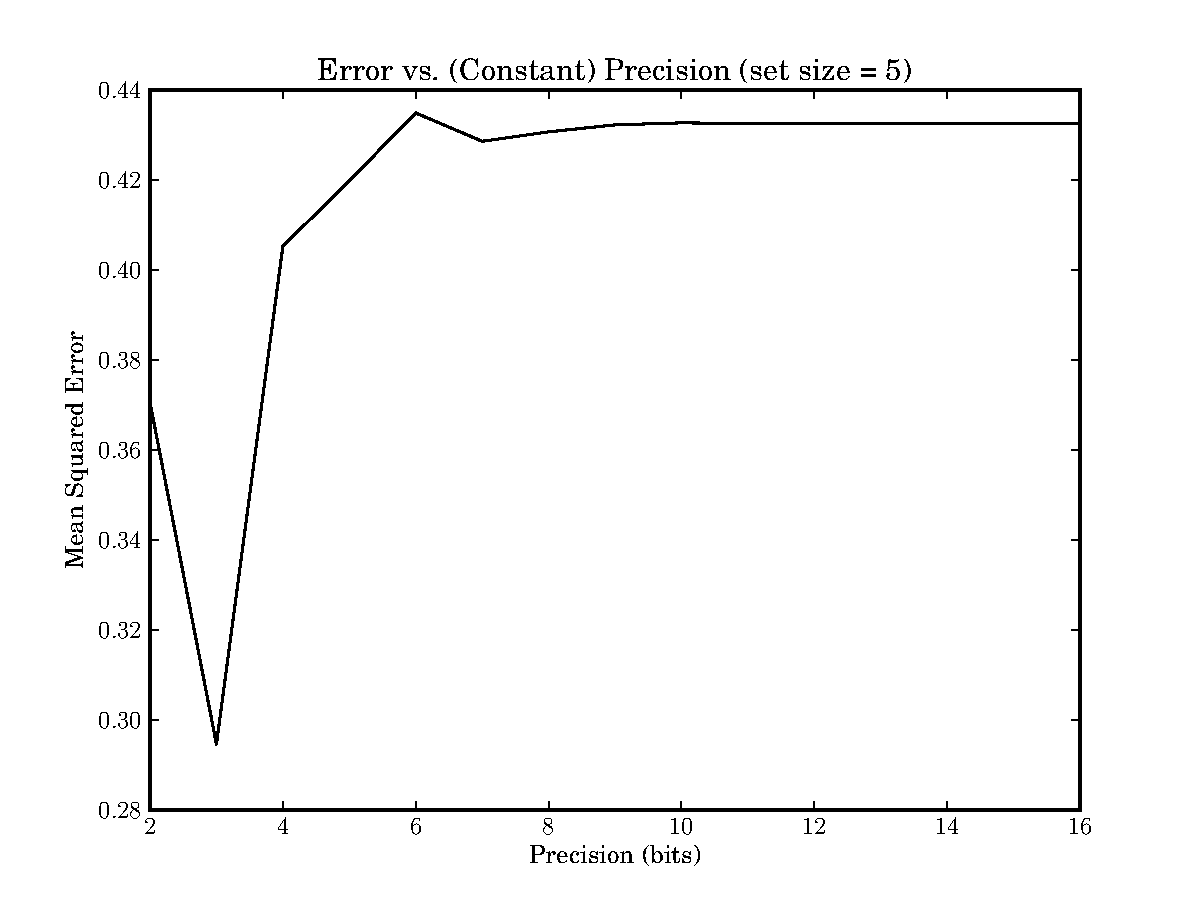
\includegraphics[scale=0.7]{error-vs-prec-ss5}
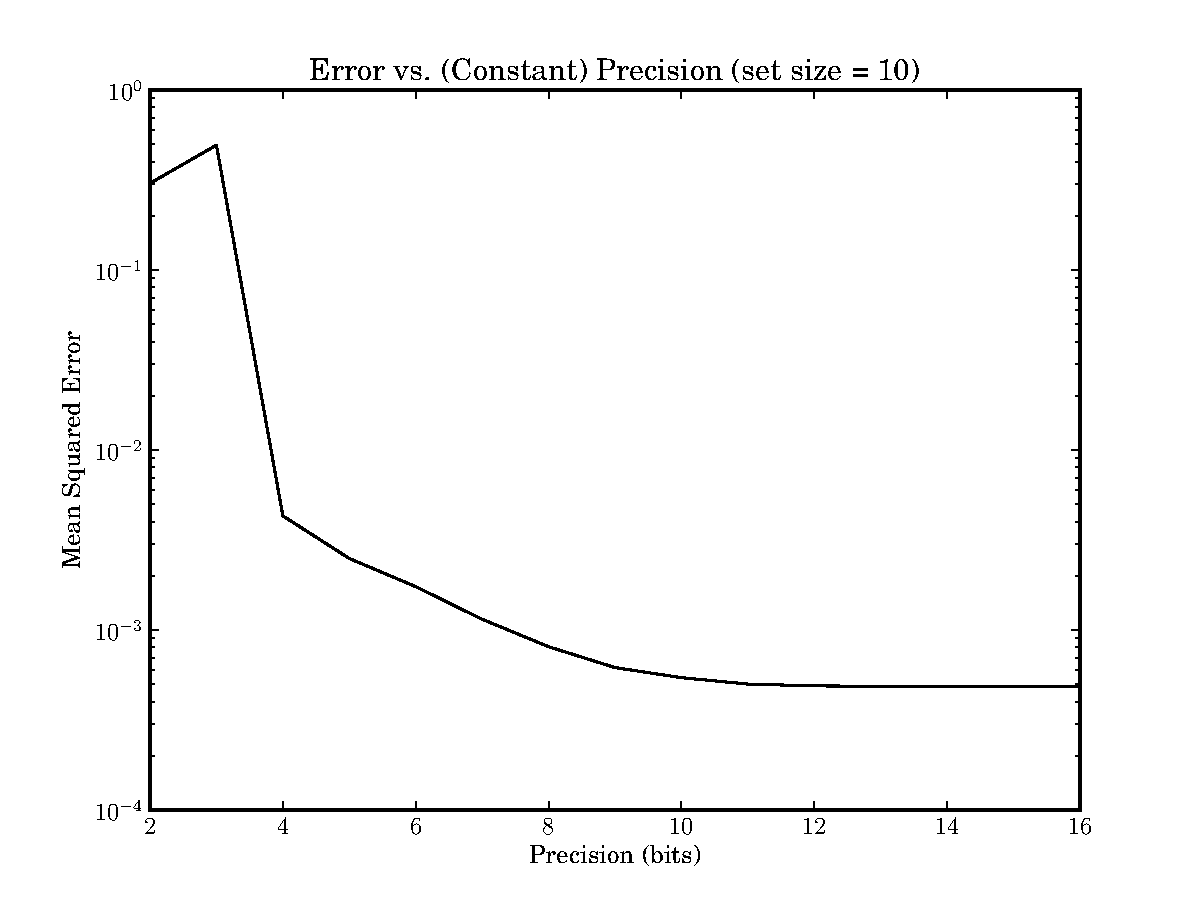
\includegraphics[scale=0.7]{error-vs-prec-ss10}
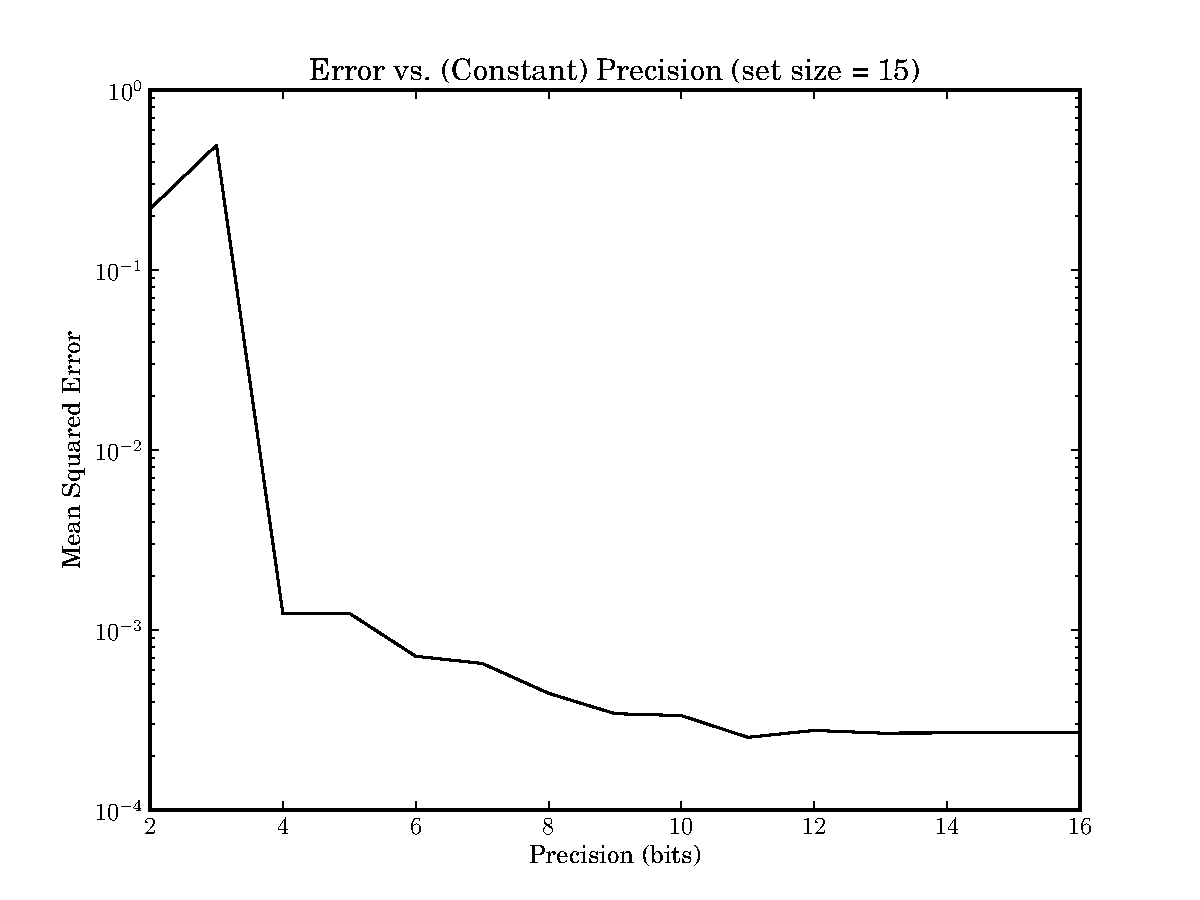
\includegraphics[scale=0.7]{error-vs-prec-ss15}
\end{center}
\end{document}
